\documentclass[paper=a4, fontsize=11pt]{scrartcl} % A4 paper and 11pt font size

\usepackage[T1]{fontenc} % Use 8-bit encoding that has 256 glyphs
\usepackage[french]{babel} % English language/hyphenation
\usepackage{amsmath,amsfonts,amsthm} % Math packages
\usepackage[utf8]{inputenc}
\usepackage{slash box}
\usepackage{graphicx}
\usepackage{sectsty} % Allows customizing section commands

\usepackage{fancyhdr} % Custom headers and footers
\pagestyle{fancyplain} % Makes all pages in the document conform to the custom headers and footers
\fancyhead{} % No page header - if you want one, create it in the same way as the footers below
\fancyfoot[L]{} % Empty left footer
\fancyfoot[C]{} % Empty center footer
\fancyfoot[R]{\thepage} % Page numbering for right footer
\renewcommand{\headrulewidth}{0pt} % Remove header underlines
\renewcommand{\footrulewidth}{0pt} % Remove footer underlines
\setlength{\headheight}{13.6pt} % Customize the height of the header


%----------------------------------------------------------------------------------------
%	TITLE SECTION
%----------------------------------------------------------------------------------------

\newcommand{\horrule}[1]{\rule{\linewidth}{#1}} % Create horizontal rule command with 1 argument of height

\title{	
  \normalfont \normalsize 
  \textsc{ENSIMAG, 2A MMIS} \\ [25pt] % Your university, school and/or department name(s)
  \horrule{1pt} \\[0.5cm] % Thin top horizontal rule
  \huge TP Traitement de l'Image\\ % The assignment title
  \horrule{1pt} \\[0.5cm] % Thick bottom horizontal rule
}

\author{\textsc{Donzeau} Anaïs\\ \textsc{Bélot} Matthieu} % Your name

\date{\normalsize\today} % Today's date or a custom date

\begin{document}

\maketitle % Print the title

\begin{center}
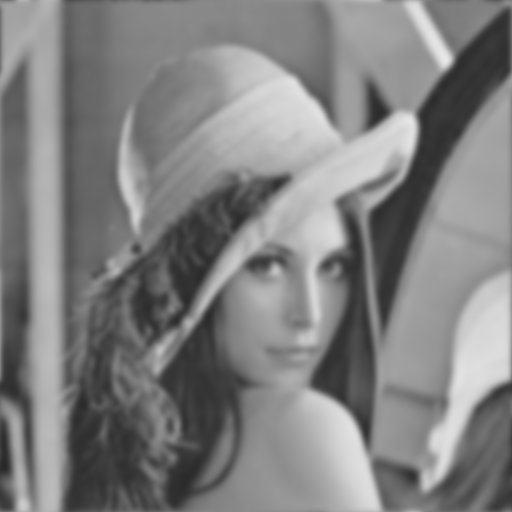
\includegraphics[width=.35\textwidth]{images/rapport/intro/coucou1.png} 
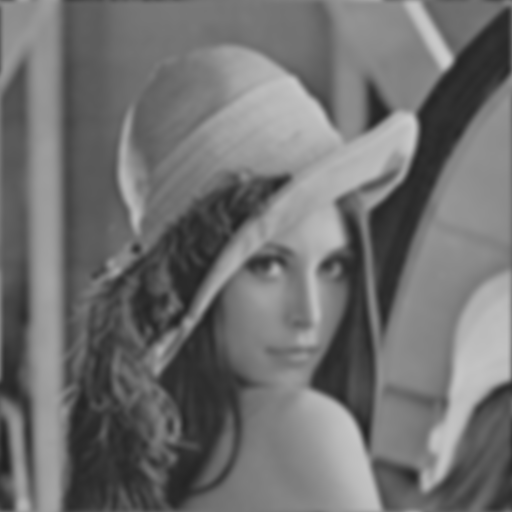
\includegraphics[width=.35\textwidth]{images/rapport/intro/coucou2.png} 
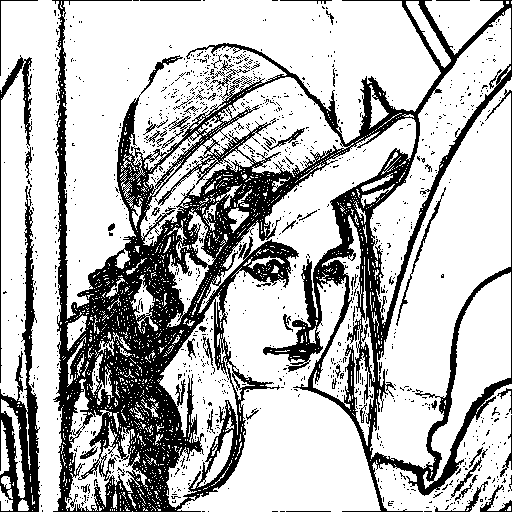
\includegraphics[width=.35\textwidth]{images/rapport/intro/coucou3.png} 
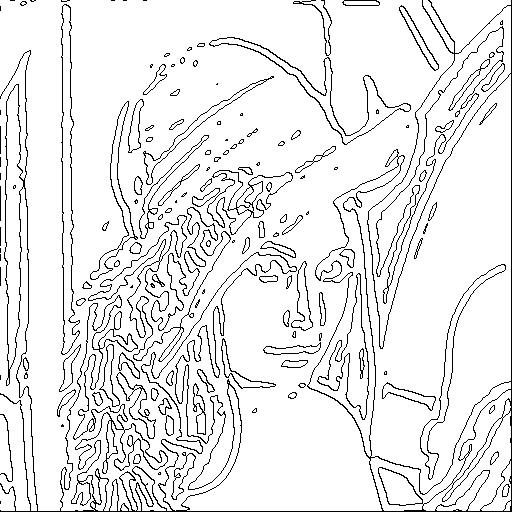
\includegraphics[width=.35\textwidth]{images/rapport/intro/coucou4.png} 
\end{center}


%----------------------------------------------------------------------------------------
%	PROBLEM 1
%----------------------------------------------------------------------------------------
\newpage
\section{Lissage linéaire}
\subsection{FFT et filtrage fréquentiel}
Ce filtrage est implémenté dans le fichier \texttt{tp1.c} avec la fonction \texttt{lissage\_temporel(char* imgOrigin, char* imgCible, double sigma)}. 

Nous avons fait le choix de mettre $\sigma$ en argument de cette fonction dans l'optique qu'un futur utilisateur puisse faire varier ce paramètre facilement. 

Le principe de ce lissage est de multiplier la FFT de l'image par la FFT de Gauss. Et le paramètre $\sigma$ est lié à la quantité de points pris autours pour la FFT. 

Les tests suivants sont basés sur 3 images : formes1pets1.pgm, formes1pets5.pgm, formes1pets10.pgm. Pour chaque image, nous avons mesuré le PSNR entre l'image d'origine et l'image avec le bruit avec différents $\sigma$. Nous avons sélectionné ce type de bruit parfaitement arbitrairement. Nous testeront l'efficacité selon le bruit ensuite. 


Par exemple, à la figure \ref{3images} pour $\sigma=2$ voici l'image bruitée (gauche) puis l'image bruitée après lissage (milieu) et l'image sans bruit utilisée comme référence pour le calcul de PSNR (droite)

\begin{figure}[h!]

\label{3images}
\caption{Image bruitée -  Image bruitée après lissage  - Image d'origine}
\centering
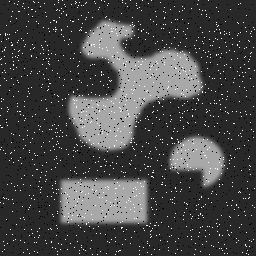
\includegraphics[scale=0.53]{images/rapport/formes1pets1.png} 
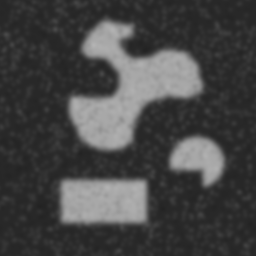
\includegraphics[scale=0.53]{images/rapport/temporel_pets1sig2.png}

\includegraphics[scale=0.53]{images/rapport/formes1.png}  
\end{figure}

\begin{table}[h!]
\caption{PSNR obtenu en fonction de l'image et de $\sigma$}
\begin{tabular}{|l|c|c|c|c|c|c|}

	\hline
	\backslashbox{$\sigma$}{Numéro image} & 1 & 5 & 10 & Observations\\ 
	\hline
	
	0.5 & 21.520569 & 15.442793 & 12.690174 & image quasiment inchangée \\
	\hline
	1 & 24.495013 & 18.941417 & 15.683970 & encore beaucoup de bruit\\
	\hline
	2 & 25.063695 & 20.419597 & 16.958596 &  disparition globale du bruit \\
	\hline
	5 & 22.822663 & 19.810204 & 16.851957 & image flou mais forme visible \\ 
	\hline
	10 & 20.105781  & 18.186184 & 16.005382 & image très flou \\
	\hline

\end{tabular}

\end{table}
On observe qu'un faible $\sigma$ ne modifie pas l'image de manière visible, ce qui est normal car on ne moyenne pas assez avec les pixels autours. Ainsi, plus au augmente sigma, plus le bruit disparaît et l'image se lisse au détriment de la netteté de l'image car on mixte une trop grande quantité de pixels autours. Il est donc important de trouver un équilibre entre l'élimination du bruit et la netteté de l'image. Avec la figure \ref{tracer1} on voit qu'autour de $\sigma=2$ on trouve le meilleur compromis pour la base d'images tests.

\begin{figure}[h!]
\centering
\caption{PSNR des images en fonction de $\sigma$}
\label{tracer1}
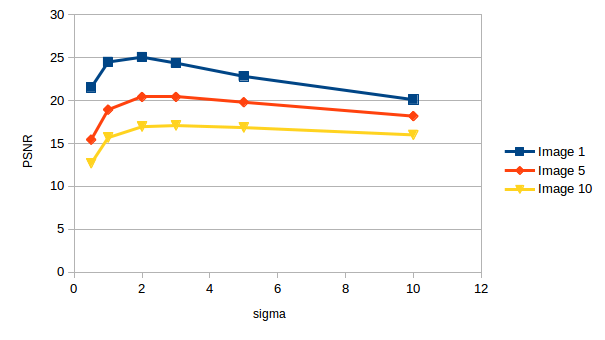
\includegraphics[scale=1]{images/rapport/courbes/pnsr1.png}
\end{figure}


\newpage

\textbf{Comparaison de l'efficacité du lissage sur les différents bruits}

Les images \texttt{formes2*.pgm} sont idéales pour effectuer ces tests car elle comporte l'image bruitée de trois manières différentes. Comme nous avons observé que $\sigma=2$ était un très bon candidat pour ce lissage, nous sommes restés sur cette valeur.

\paragraph{Bruit Poivre et Sel}
Pour le bruit de type Poivre et Sel on obtient le lissage à la figure \ref{PETS2}.

\begin{figure}[h!]
\caption{Avant lissage / Après lissage}
\label{PETS2}
\centering
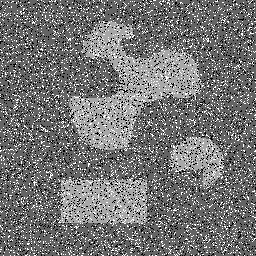
\includegraphics[scale=0.6]{images/rapport/pets/formes2pets5.png} 
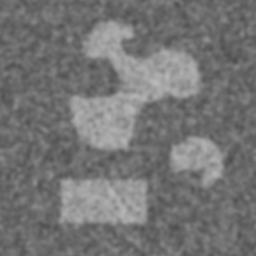
\includegraphics[scale=0.6]{images/rapport/pets/pets5sig2.png}
\end{figure}

\paragraph{Bruit Gaussien}
Pour le bruit de type Gaussien on obtient le lissage à la figure \ref{BB2}.

\begin{figure}[h!]
\caption{Avant lissage / Après lissage}
\label{BB2}
\centering
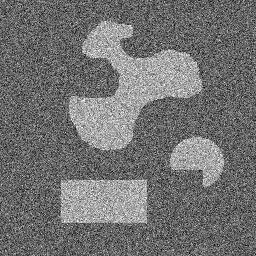
\includegraphics[scale=0.6]{images/rapport/bb/formes2bb30.png} 
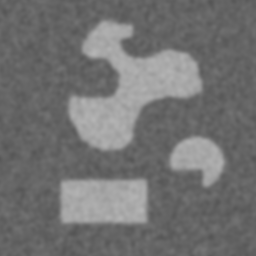
\includegraphics[scale=0.6]{images/rapport/bb/bb30.png} 
\end{figure}

\paragraph{Bruit Speckle}
Pour le bruit de type Speckle on obtient le lissage à la figure \ref{SP2}.

\begin{figure}[h!]
\caption{Avant lissage / Après lissage}
\label{SP2}
\centering
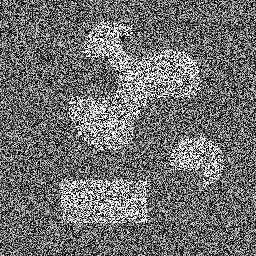
\includegraphics[scale=0.6]{images/rapport/sp/formes2sp5.png} 
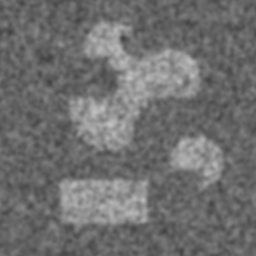
\includegraphics[scale=0.6]{images/rapport/sp/sp5sig2.png} 
\end{figure}


D'un point de vue qualitatif, le lissage fréquentiel semble plus efficace sur le bruit Gaussien et bien moins efficace sur le bruit Speckle. 

A la table \ref{typebruitpnsr}, on peut voir que le PSNR de l'image lissée en fonction de son bruit initial.

\begin{table}
\caption{PSNR de l'image lissée en fonction de bruit initial}
\label{typebruitpnsr}
\centering
\begin{tabular}{|l|c|c|c|}
\hline
	\backslashbox{$\sigma$}{Type de bruit} & Gaussien & Poivre et Sel & Speckle \\
	\hline
	2 & 31.244236 & 26.025110 & 25.099823 \\
	\hline
	5 & 28.972213 & 26.217272 & 25.911760 \\
	\hline
\end{tabular}

\end{table}

On observe donc, qualitativement et quantitativement, que le lissage fréquentiel est très efficace sur le bruit Gaussien et bien moins efficace sur un bruit Poivre et Sel et Speckle. 

En conclusion, cette méthode fourni des résultats plutôt bons à condition d'avoir trouvé la valeur $\sigma$ pour laquelle on obtient le meilleur compromis entre netteté et élimination du bruit. En figure \ref{avantapresglobules}, on peut voir un avant/après d'une images de globules. On observe une élimination efficace du bruit après lissage.

\begin{figure}[h!]
\centering
\caption{Avant/après lissage d'une image de globules}
\label{avantapresglobules}
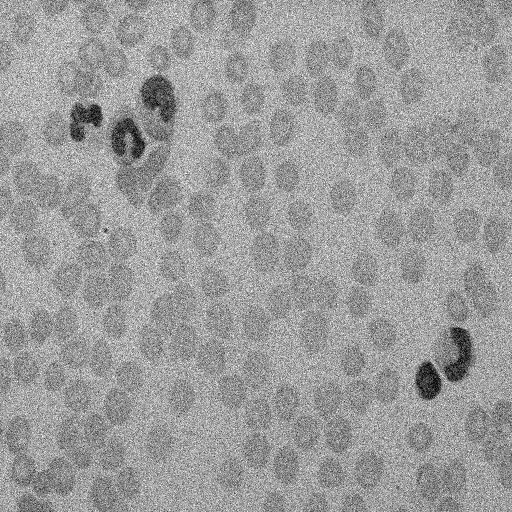
\includegraphics[scale=0.3]{images/rapport/globulesav.png} 
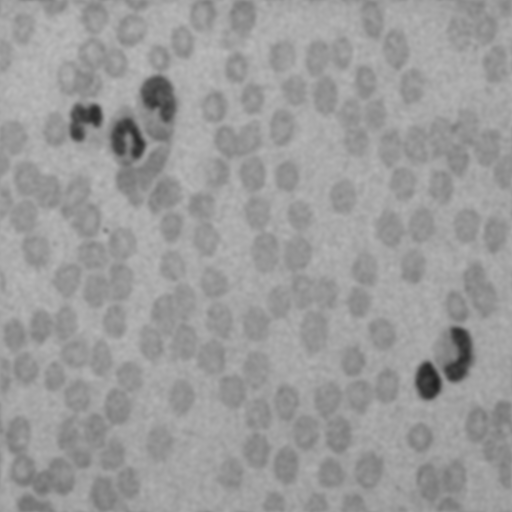
\includegraphics[scale=0.3]{images/rapport/globules2.png}
\end{figure}

\newpage
\subsection{Convolution spatiale}
Ce filtrage est implémenté dans le fichier \texttt{tp1.c} avec la fonction \texttt{lissage\_spatial(char* imgOrigin, char* imgCible, double sigma, int n, int m)}.

Nous avons fait le choix de mettre $\sigma$ ainsi que la taille de masque $n*m$ en argument de cette fonction dans l'optique qu'un futur utilisateur puisse faire varier ces paramètres facilement.\\

L'image lissée est le résultat d'un produit de convolution entre l'image et un masque. La taille du masque permet de définir la quantité de pixels qui seront pris autour du pixel lissé. Le paramètre $\sigma$ a la même fonction que pour le lissage précédent. \\

\textbf{Comparaison avec le lissage fréquentiel}

Afin d'obtenir la loi empirique $W(\sigma)$ nous nous sommes basés sur les images \texttt{formes1pets[1/5/10].pgm}. Nous avons procédé de la manière suivante :
\begin{enumerate}
\item Lissage fréquentiel et temporel des images pour différentes tailles de masques et différents $\sigma$
\item Appel d'un programme calculant le PSNR entre les images obtenues
\item Pour chaque $\sigma$ on a sélectionné la taille du masque où le PSNR était maximal, cela correspond à la taille du masque pour laquelle les résultats sont identiques par FFT et par lissage spatial. Nous avons ensuite tracé le résultat.
\end{enumerate}
Pour les étapes 1 et 2 nous avons adapté le programme à une utilisation par script (cf le fichier \texttt{tp1\_pourtest.c} entrée à l'exécution : \{Nom de l'image d'origine\} \{Nom de l'image avec lissage fréquentiel\} \{Nom de l'image avec lissage spatial\} \{N\} \{M\} \{$\sigma$\} où N*M correspond à la taille du masque) et nous avons donc rédigé un script \texttt{generator.sh} permettant d'exécuter le programme sur une liste d'image, de $\sigma$ et de taille de masque donnée puis de mesurer le PSNR entre les deux images obtenues. 

Les figures \ref{w(sig)pets1}, \ref{w(sig)pets5} et \ref{w(sig)pets10} montrent les tracés de la loi empirique.
On observe une tendance linéaire pour les trois courbes obtenues.


\begin{figure}[h!]
\centering
\caption{Tracer de $W(\sigma)$ pour l'image \textit{formes1pets1.pgm}}
\label{w(sig)pets1}
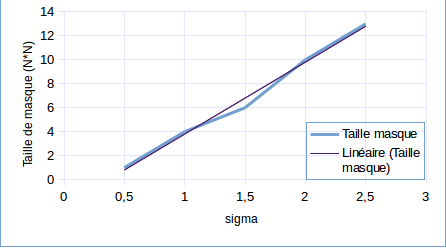
\includegraphics[scale=0.8]{images/rapport/courbes/img1W.png} 
\end{figure}

\begin{figure}[h!]
\centering
\caption{Tracer de $W(\sigma)$ pour l'image \textit{formes1pets5.pgm}}
\label{w(sig)pets5}
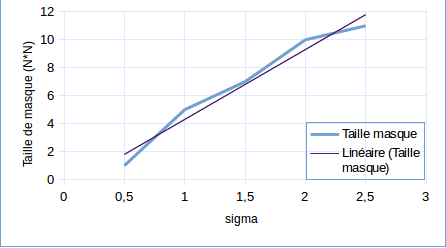
\includegraphics[scale=0.8]{images/rapport/courbes/img5W.png} 
\end{figure}

\begin{figure}[h!]
\centering
\caption{Tracer de $W(\sigma)$ pour l'image \textit{formes1pets10.pgm}}
\label{w(sig)pets10}
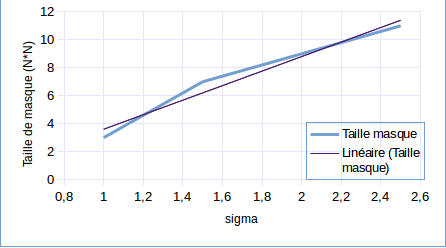
\includegraphics[scale=0.8]{images/rapport/courbes/img10W.png} 
\end{figure}

On obtient une courbe de la forme $A\sigma + B$ avec $A \in [5,6] et B\in[0.7,2.2]$. La variation du coefficient directeur et de l'ordonnée à l'origine ne sont pas abbérants.
Ainsi, on considère la loi empirique comme étant : 
\begin{center}
$W(\sigma) = A*\sigma+B$
\end{center}

Ainsi, pour un $\sigma$ donné il faut un masque de taille $\sim 5*\sigma$. Cependant, qualitativement, on ne voit plus de différence à partir d'un masque de taille $\sim 3*\sigma$. 

Les résultats de lissage sur les images de différents bruit donc totalement similaires à celles obtenues pour le lissage fréquentiel en figure \ref{SP2}, \ref{PETS2} et \ref{BB2}.
\subsection{Complexité est comparaison des deux méthodes}
Pour mesurer le temps de calcul en fonction de $\sigma$ nous avons pris un masque égale à $6x6$ car celui-ci obtient de bons résultats (qualitativement parlant) pour de nombreux $\sigma$. Dans ce cas nous obtenons le résultat en figure \ref{tempscalculsigma}.

On observe que le temps de calcul varie très peu en fonction de $\sigma$. On peut donc considérer que $\sigma$ n'a pas d'impact sur le temps de calcul. On observe par ailleurs que l'écart entre le temps de calcul de l'image lissée par le lissage fréquentiel et spatial est très significatif. Le lissage spatial est nettement plus long que le lissage temporel.


\begin{figure}
\caption{Temps de calcul en fonction de $\sigma$ pour un masque de taille 6$\times$6}
\label{tempscalculsigma}
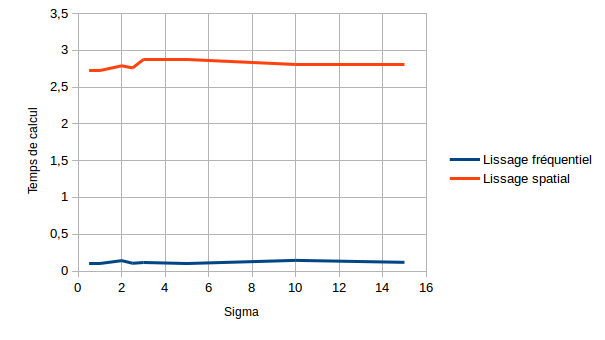
\includegraphics[scale=1]{images/rapport/courbes/temps_calcul_sigma.png} 
\end{figure}

Afin de vérifier si cette hypothèse est valable pour n'importe quelle taille de masque, nous avons tracé pour $\sigma=2.0$ le temps de calcul en fonction de la taille du masque (en $n \times n$) en figure \ref{tempscalculmasque}. Bien sûr, le lissage fréquentiel ne dépend pas de la taille du masque, donc il est constant. Ce qui est plus intéressant est de voir l'écart entre le temps de calcul du lissage fréquentiel et spatial qui est de plus en plus grand suivant la taille du masque. 

En exploitant les résultats, on pourrait dire qu'à partir d'une masque de taille $0.6\times0.6$ il est plus rapide de faire le lissage fréquentiel que spatial. Cependant prendre un masque de taille $<1$ n'a pas vraiment de sens vu qu'on prend des pixels. Ainsi, le lissage fréquentiel est toujours plus rapide que le lissage spatial et, pour des masque de petite taille ($\sim <2$), l'écart de temps de calcul n'est pas très grand mais les résultats ne sont pas aussi bons en lissage spatial qu'en lissage fréquentiel.


En conclusion, nous avons deux méthodes de lissages qui ont le même effet sur les images et réagissent très bien à un bruit Gaussien et légèrement moins bien sur un bruit Poivre et Sel ou Speckle. Le lissage spatial est nettement plus long que le lissage fréquentiel mais permet une meilleure liberté sur le résultat souhaité avec les deux paramètres définissant la taille du masque. 

\begin{figure}
\caption{Temps de calcul en fonction de la taille du masque $n \times n$ pour $\sigma=2.0$}
\label{tempscalculmasque}
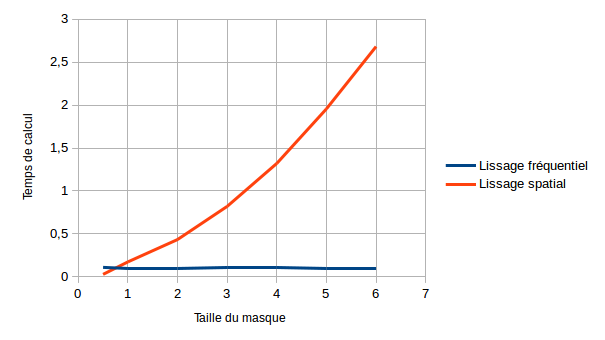
\includegraphics[scale=1]{images/rapport/courbes/temps_calcul_masque.png} 
\end{figure}

\section{Détection de contours}

\subsection{Opérateur différentiel du premier ordre}
Pour détecter les contours, nous avons utilisé le gradient de Sobel qui donne un peu plus d'importance aux pixels adjacents qu'au pixel diagonaux

On peut observer en figure \ref{Contour1ordre} le résultat d'une détection de contours avec ce modèle. Le résultat semble sensible au bruit car on voit quelques contours parasites mais on voit très clairement le contour de l'image.

\begin{figure} [h!]
\caption{Image d'origine / Détection de contours}
\label{Contour1ordre}
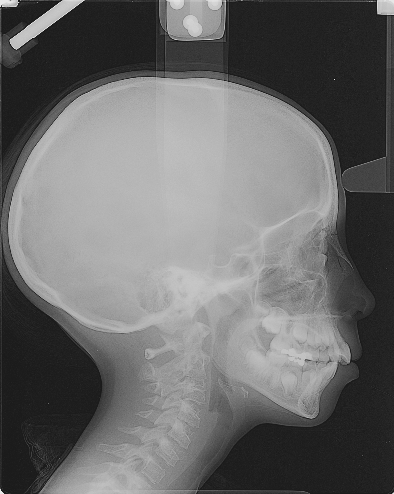
\includegraphics[scale=0.5]{images/rapport/radio1.png} 
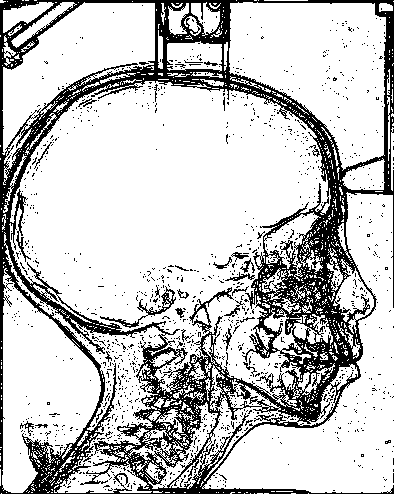
\includegraphics[scale=0.5]{images/rapport/coucou1.png} 
\end{figure}



\subsection{Opérateur différentiel du deuxième ordre}
\subsubsection{LoG}
\subsubsection{FFT}



LOG lent 1er ordre rapide
\end{document}